\chapter{Intention Oriented Organizational Modeling}
\label{chap:orgModeling}

%%%%%%%%%%%%%%%%%%%%%%%%%%%%%%%%%%%%%%%%%%%%%%%%%%%%%%%%%%%%%%%%%%%%%%%%%
\section{Overview and Modeling process}
%%%%%%%%%%%%%%%%%%%%%%%%%%%%%%%%%%%%%%%%%%%%%%%%%%%%%%%%%%%%%%%%%%%%%%%%%
\hspace{4ex} The Organizational Modeling element notation has been selected as per the guidelines mentioned in the paper by Moody \cite{Moody2009}. Also by observing  the fact that business process modelers are already well-known with the present process modeling notations such as Business Process Modeling Notation 2.0 (BPMN) \cite{bpm2011} and ArchiMate notation\cite{arc2013}, the shape depiction of organizational model elements are designed similar to those existing process notations. 





%%%%%%%%%%%%%%%%%%%%%%%%%%%%%%%%%%%%%%%%%%%%%%%%%%%%%%%%%%%%%%%%%%%%%%%%%
\section{Organizational Modeling Notation}
%%%%%%%%%%%%%%%%%%%%%%%%%%%%%%%%%%%%%%%%%%%%%%%%%%%%%%%%%%%%%%%%%%%%%%%%%
\hspace{4ex} Due to the importance of shapes in expressing the information visually , the notations are chosen in such a way that each element of Organizational Modeling  differ by shape. Also a legend will be always shown in the modeling notation to denote the meaning of each shape \cite{Moody2009}. As shape plays a primary role in discriminating between different element, organizational model notations are represented through individual shapes like rectangle, double circle, elliptic etc.,. The description of each element in the Organizational Model Notation is shown in the Table \ref{tab:notations}. 

\begin{center}
	\begin{longtable}{p{3cm}p{10cm}p{3cm}}
		\toprule 
		\textbf{Element} & \textbf{Definition} & \textbf{Notation} \\
		\midrule
		\endfirsthead
		Intention 			& Intentions are purposeful concrete steps taken to achieve expected outcomes . They reflect the actual intention of an organization.Intentions are defined hierarchically, which can contain and extend intentions.It is depicted by a double circle. The sub-intentions are refined starting from main intention. intentions associated with capabilities are concrete intentions and intentions that are not associated with capabilities are abstract intentions. Abstract intentions are represented by dashed double circle and concrete intentions are depicted by a solid double circle. & \begin{center} 
\includegraphics[width= 0.07\textwidth]{intentions.png}  \end{center}  \\  
		
		Capabilities	& Organizational capability is the ability to provide business values like software applications, resources, and potential of the actor to make decisions even in changing situations \cite{Stirna2012}. Capabilites are represented by a elliptical circle. Capability is an ability that should be possessed by an Actor or a Resource that work towards achievement of intention.   & \begin{center} 
\includegraphics[width= 0.1\textwidth]{capabilities.png} \end{center}   \\
		
		Context				& The environment that forms the setting for an event, statement, or idea, and in terms of which it can be fully understood. There are two Contexts: Initial and Final. The Initial Context is the situation which describes the driving forces that trigger the process to start. The Final Context is the expected situation once the process has finished.Both initial and final context are represented by an hexagonal shape except the final context has thick edges than initial context.  & \begin{center} 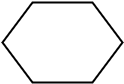
\includegraphics[width= 0.1\textwidth]{context.png} \end{center}  \\
		
		
		Strategy		&  A method or plan chosen to bring about a desired future, such as accomplishment of a intention. Strategies are expressed by rectangles with sharp edges. In the conceptual Organizational Modeling, strategies are self-contained and loosely coupled elements.   & \begin{center} 
\includegraphics[width= 0.1\textwidth]{strategy.png} \end{center}   \\
		
		Resources					& The people and tools needed to fulfill the middle objectives or those/that work towards the achievement of intention . Resources are represented by a rounded rectangle. Resources are linked to capabilities and actors. & \begin{center} 
\includegraphics[width= 0.1\textwidth]{resources.png} \end{center}   \\
		
		Actors					& People who participate in the process. Actors are represented by a stick-man and they are linked to resource as actors can be resources. Actors define the strategy and intentions.  & \begin{center} 
\includegraphics[width= 0.07\textwidth]{actor.png} \end{center}   \\
		
		Relationship				& A relationship is used specify the fixed links between the elements of the model. Relationship between two elements is represented by a single direction line which represents a sequence.  & \begin{center} 
\includegraphics[width= 0.1\textwidth]{relationship.png} \end{center}   \\
		
		
		\bottomrule
		\caption{Informal Process Modeling Notation}
		\label{tab:notations}		
	\end{longtable}	
\end{center}


%%%%%%%%%%%%%%%%%%%%%%%%%%%%%%%%%%%%%%%%%%%%%%%%%%%%%%%%%%%%%%%%%%%%%%%%%
\section{Organizational Modeling Notation Example}
%%%%%%%%%%%%%%%%%%%%%%%%%%%%%%%%%%%%%%%%%%%%%%%%%%%%%%%%%%%%%%%%%%%%%%%%%
\hspace{4ex} The concept of Organizational Model Notations can be explained with the following manufacturing scenario. ABC Ltd. is a budding computer technology company which designs, develops, manufactures and sells personal computers, tablets and laptops. The CEO's intention of the quarter is to increase the revenue and number of unit sales. The initial context describes the situation that motivates to start the process. The final context describes the situation that is achieved once the process completed successfully. intentions connect initial context definitions with final context definitions \cite{Sungur2014a}. The sub-intentions are the intermediate intentions which describes the expected outcome in a measurable form. intentions are reached through strategy implementation which is plan of action designed to meet a intention. 

\hspace{4ex} The example scenario ABC Ltd. helps in understanding the organizational modeling i.e., how organization's higher level intention can be achieved by amalgamation of specific, measurable and realistic sub-intentions. . The whole view has been divided into intention view and Strategy view. The \textit{intention View} shown in the Figure\ref{fig:intentionview} provides only the details of intention and its associated strategies. There can be multiple strategies followed to achieve a intention. The \textit{Strategy View} shown in the Figure\ref{fig:strategyview} connects big picture of each strategy with individual intentions that has to be carried out. In Organizational Process Modeling, strategies are self-contained and loosely coupled. So that when we extract only the strategies from Organization Process Modeling it would be similar to Informal Process Essential Modeling. 

\hspace{4ex} The Strategy view  in the Figure\ref{fig:strategyview} depicts big picture of each strategy. Strategies are associated with both intentions and capabilities. Capabilities are related to intentions and resources. As each intention needs certain capability to successfully execute the intention they both are connected using the verb \textit{"requires"}. Resources are the potential holder of the capability i.e., to satisfy a capability we need resources. The capability and its associated resources are linked using the verb \textit{"satisfied-by"}. 


\begin{figure}
	\centering
	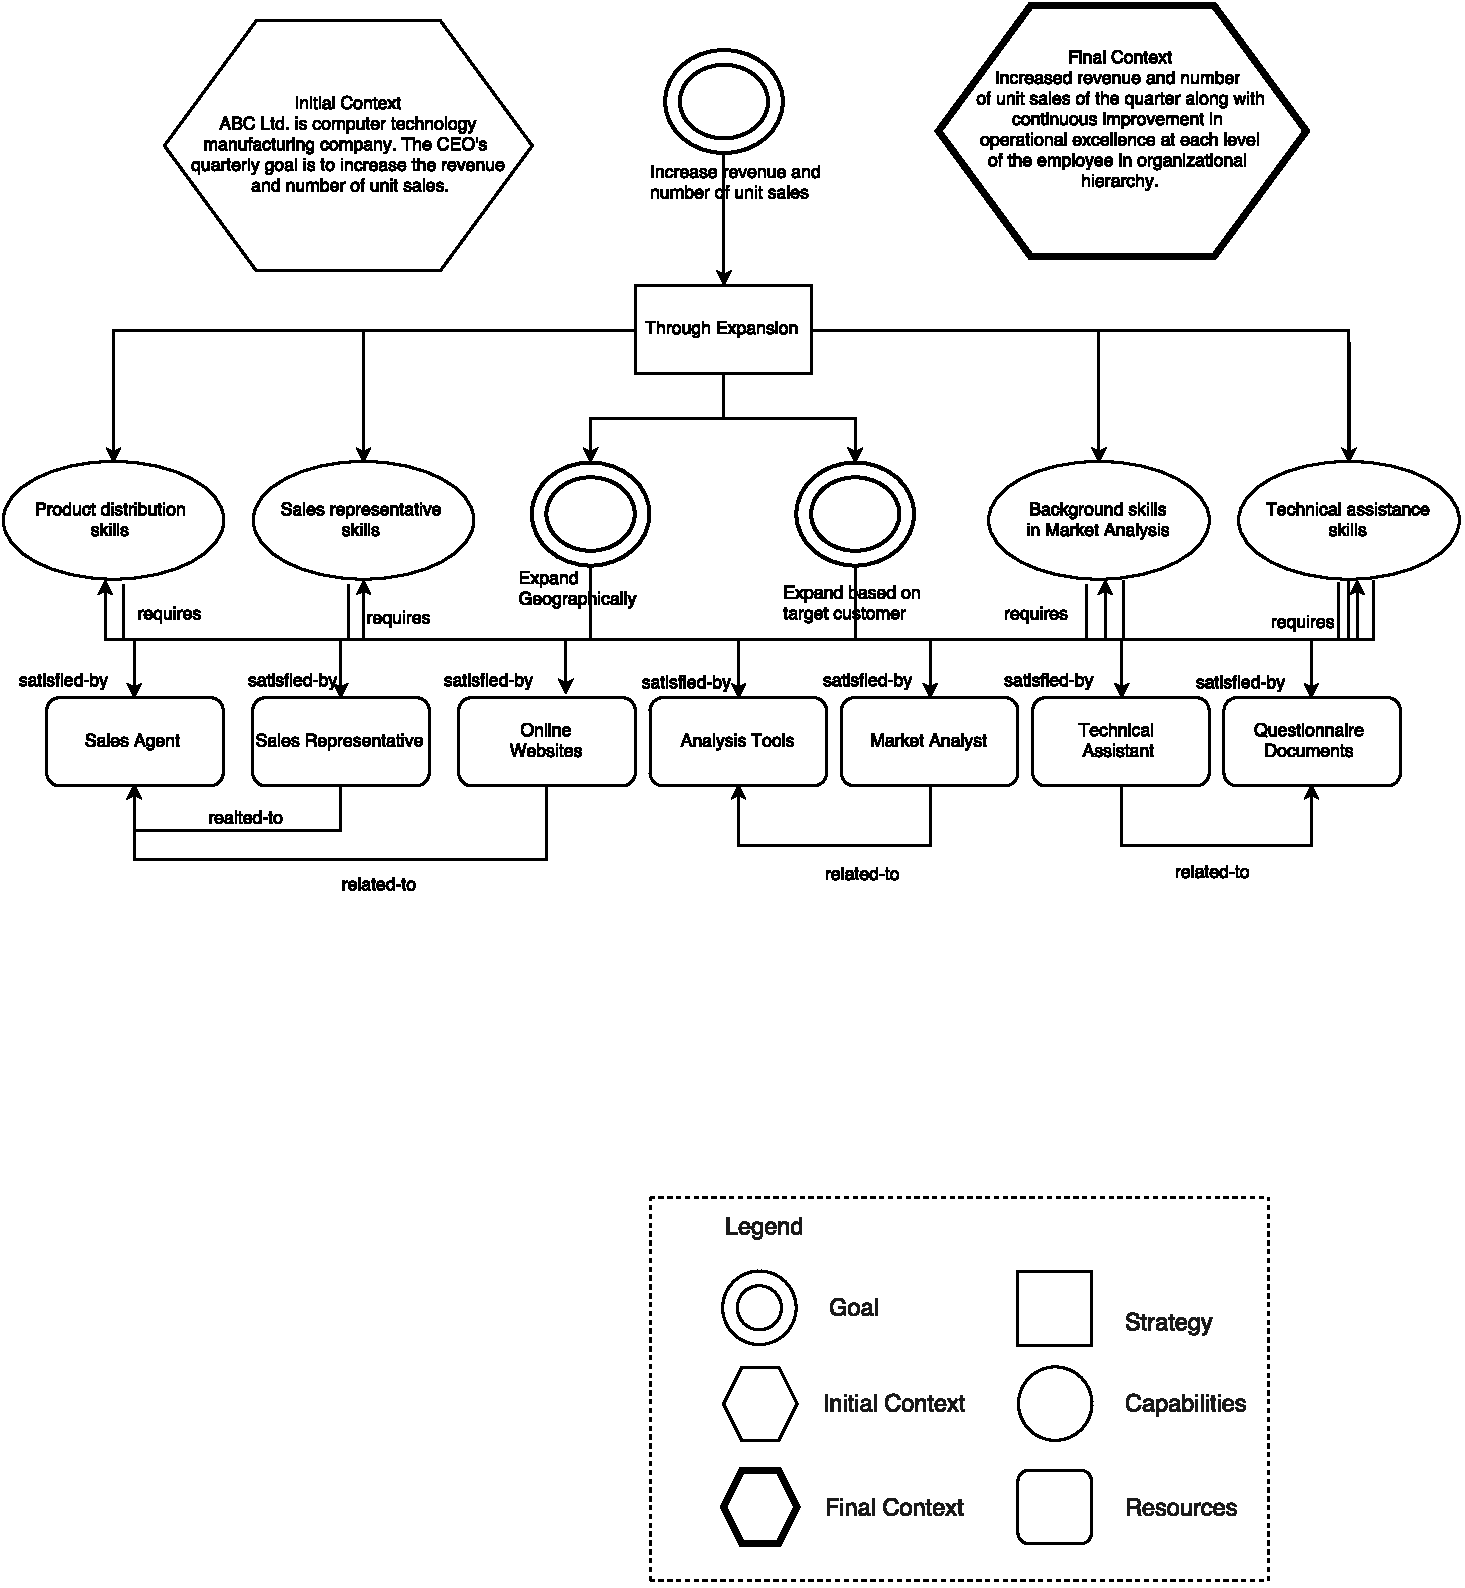
\includegraphics[width=\textwidth]{StrategyView.pdf}
	\caption{Strategy View}
	\label{fig:strategyview}
\end{figure}

\begin{figure}
	\centering
	\includegraphics[width=\textwidth]{goalView.pdf}
	\caption{intention View}
	\label{fig:intentionview}
\end{figure}

%%%%%%%%%%%%%%%%%%%%%%%%%%%%%%%%%%%%%%%%%%%%%%%%%%%%%%%%%%%%%%%%%%%%%%%%%
\section{Organizational Modeling Process Representation}
%%%%%%%%%%%%%%%%%%%%%%%%%%%%%%%%%%%%%%%%%%%%%%%%%%%%%%%%%%%%%%%%%%%%%%%%%
\begin{figure}
	\centering
	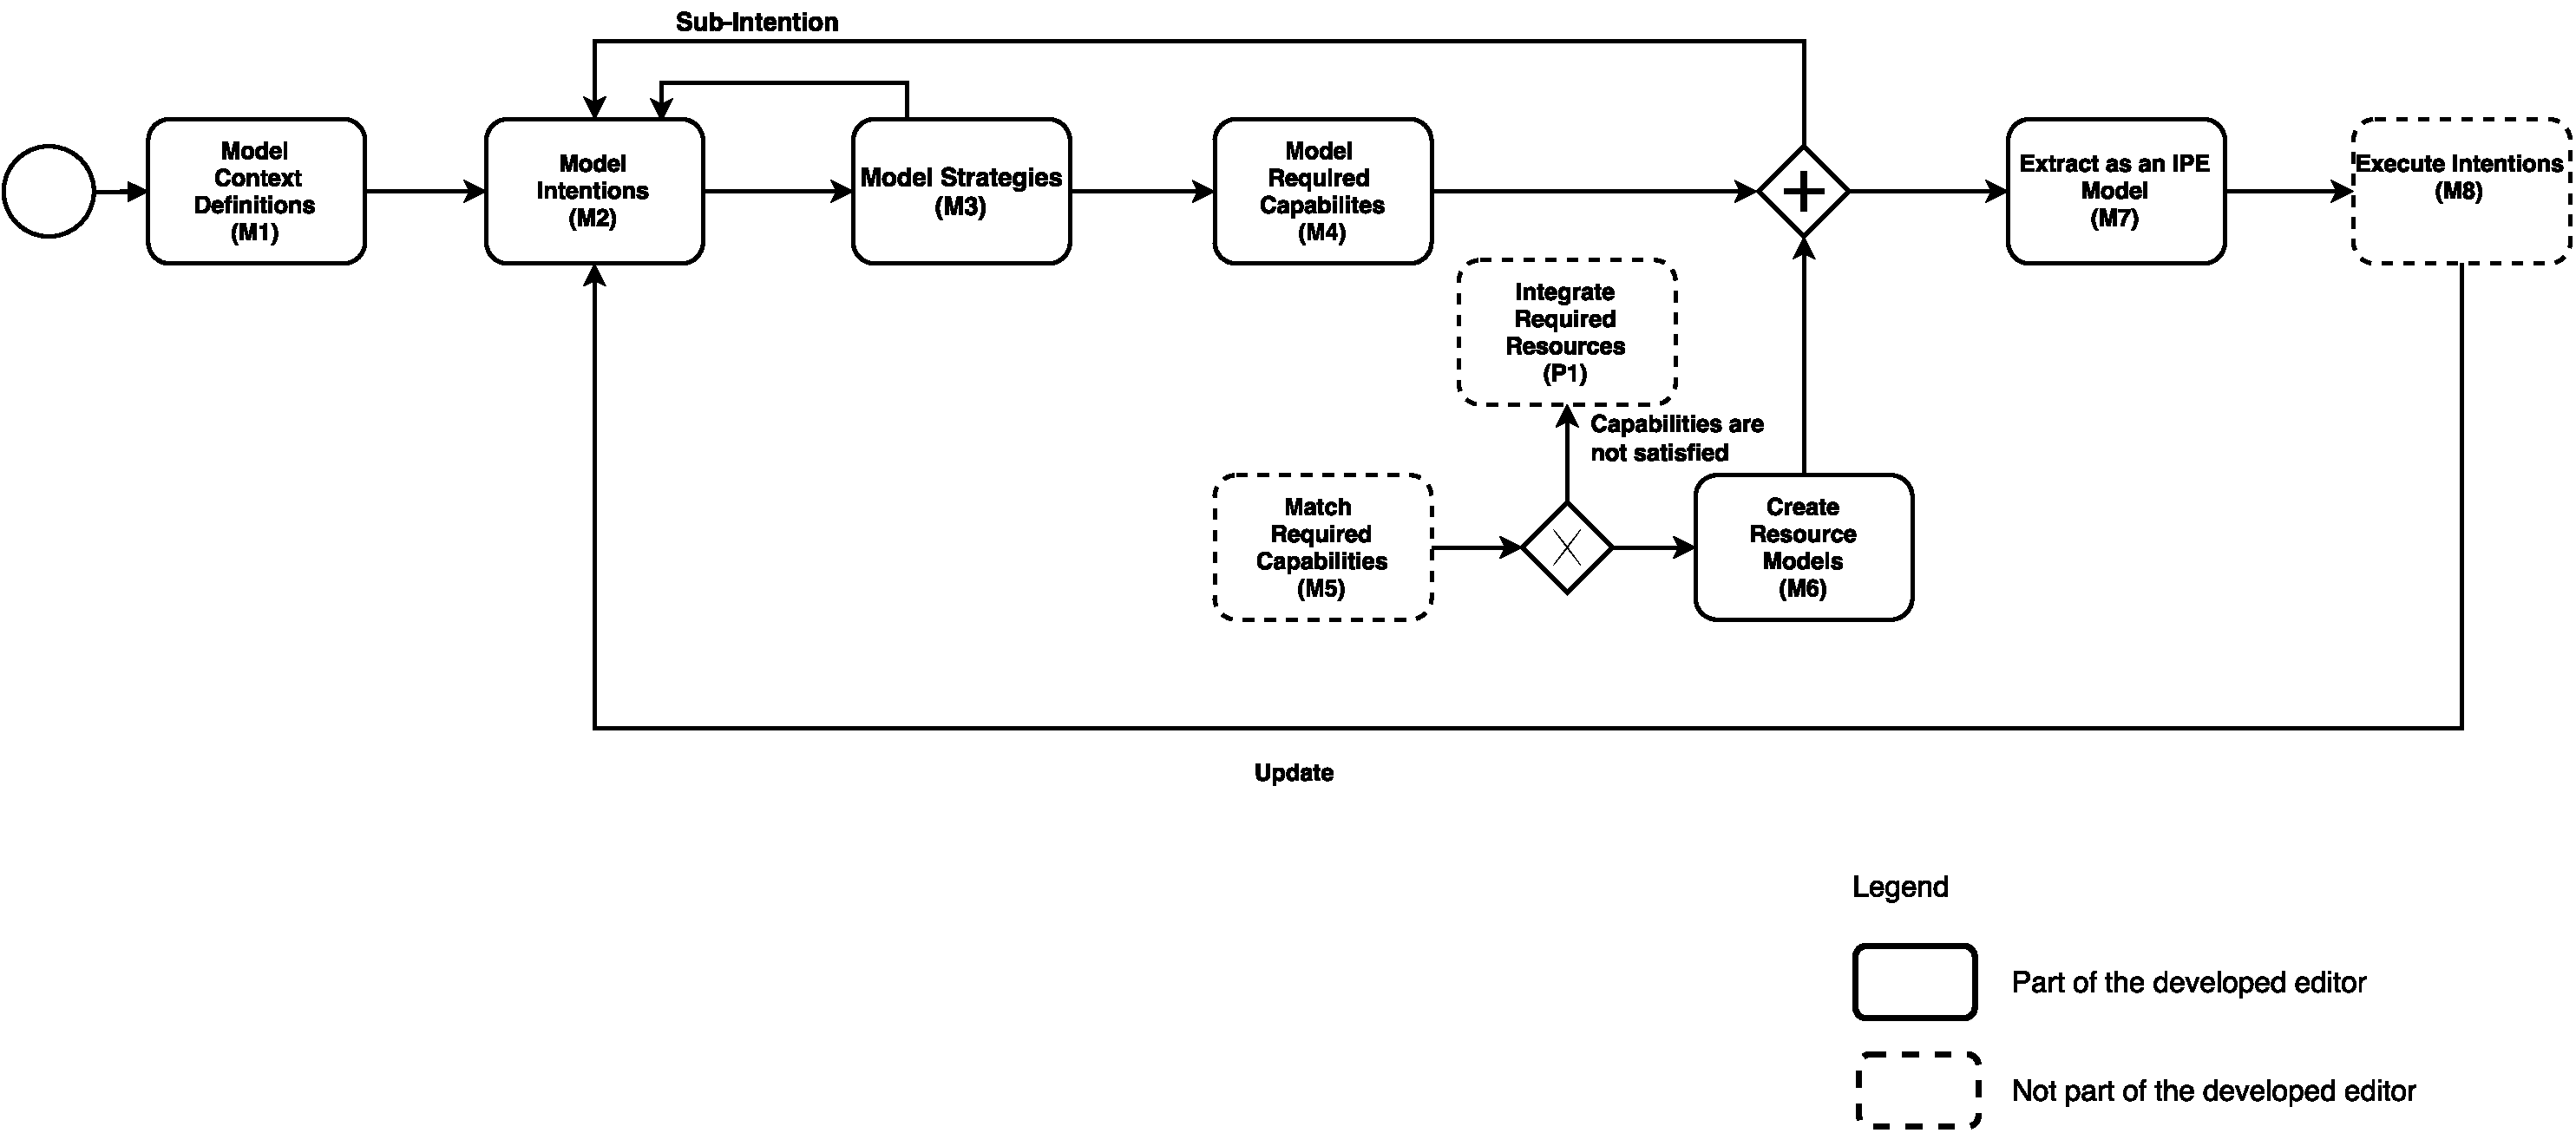
\includegraphics[width=\textwidth]{processmodeling.pdf}
	\caption{Process Modeling Diagram}
	\label{fig:processdiagram}
\end{figure}

\hspace{4ex} Organizational Process Modeling depicted inFigure \ref{fig:processdiagram} captures required organizational capabilities that are satisfied by resource models  to enable the achievement of organizational intentions in certain context definitions through a strategy. It is a top-down approach, i.e., first intentions are defined and then sub-intentions  are defined by refining main intention. intentions connect initial context definitions with final context definitions through a strategy.  To understand the definition of Organizational Process Modeling we need to interpret the Organizational Process Modeling Representation shown in Figure\ref{fig:processdiagram}. 

\hspace{4ex} The Organizational Process Modeling start with modeling of organizational intention (M1). Once the intention has been modeled, the second step is to model the strategies which can be a multi-instance strategy model(M2). The next step is to model the context definitions (M3.1), required organizational capabilities (M3.2) and refining the sub-intentions from main intention in parallel. Once the required capabilities(M4) are matched by required resources(P1), modeling of resources(M5) can be done.  Based on created resource models (M5) and modeled context definitions(M3.1), strategies can be executed. The organizational intentions would be iteratively updated supported to strategy execution.  


%%%%%%%%%%%%%%%%%%%%%%%%%%%%%%%%%%%%%%%%%%%%%%%%%%%%%%%%%%%%%%%%%%%%%%%%%
\section{Organizational Modeling Entity Representation}
%%%%%%%%%%%%%%%%%%%%%%%%%%%%%%%%%%%%%%%%%%%%%%%%%%%%%%%%%%%%%%%%%%%%%%%%%

\begin{figure}
	\centering
	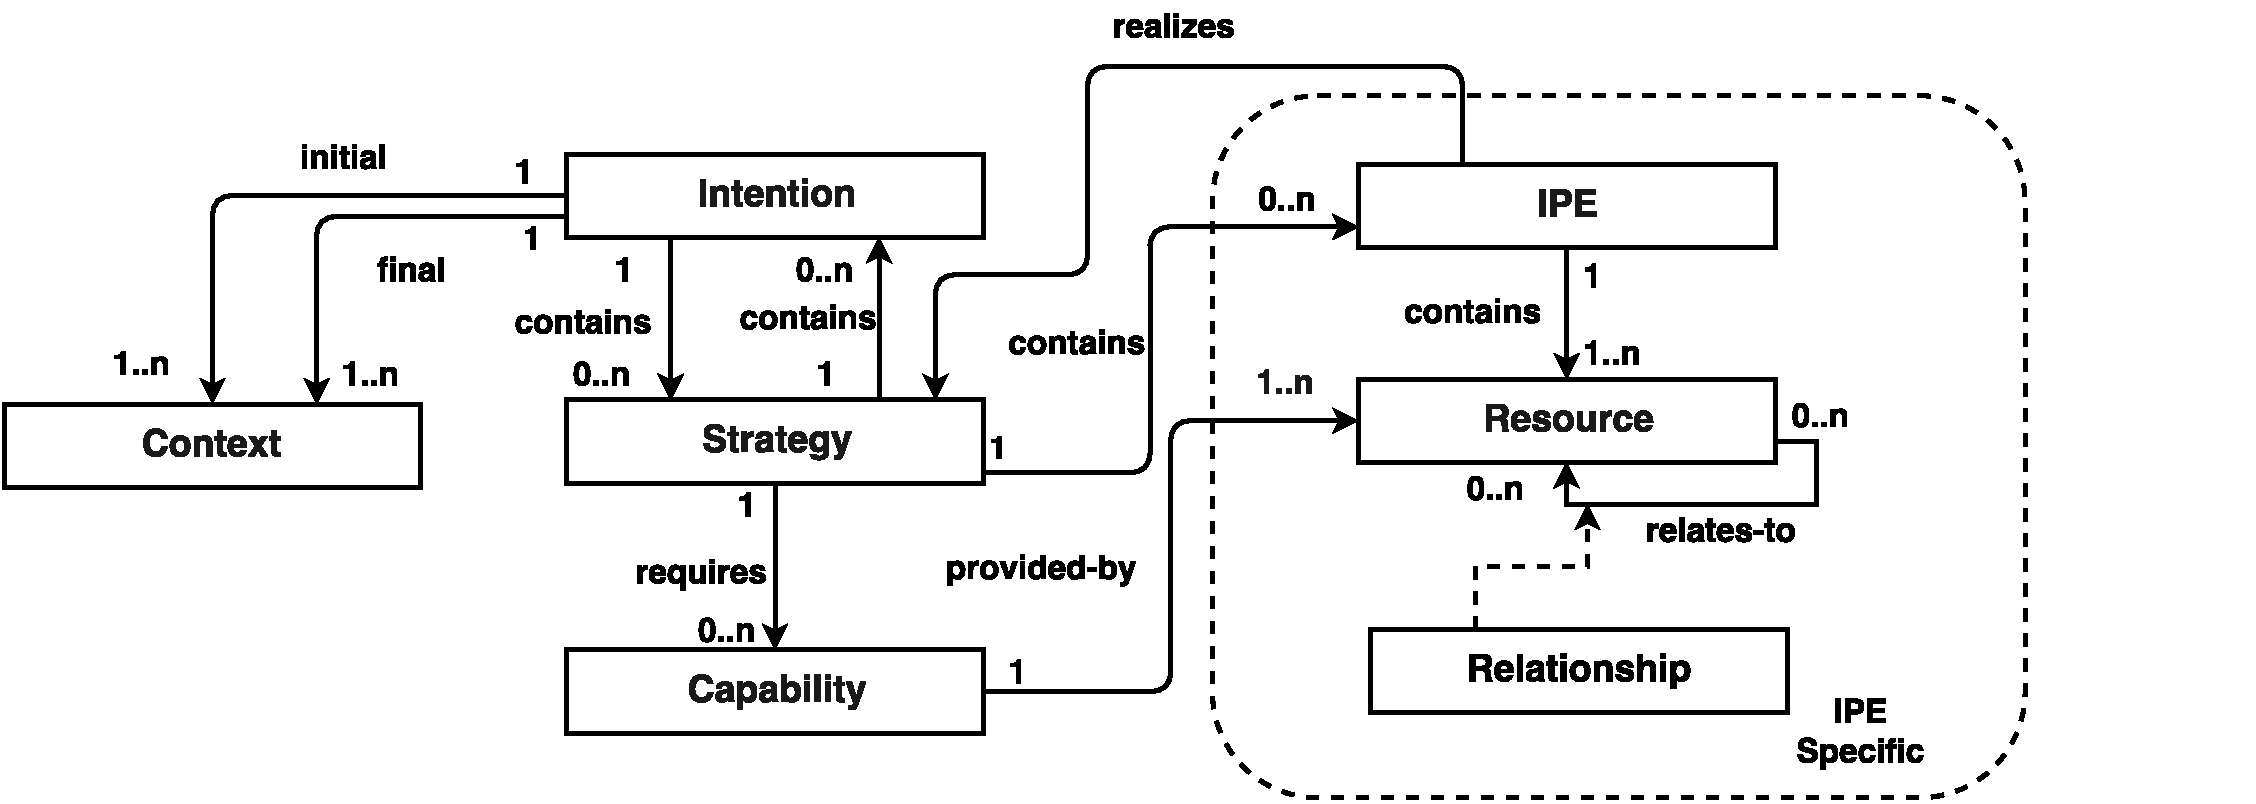
\includegraphics[width=\textwidth]{entity.pdf}
	\caption{Organizational Modelling Meta-Model}
	\label{fig:metamodel}
\end{figure}

\hspace{4ex} The conceptual entity model of intentions is shown in the \ref{fig:metamodel}. This model shows that top level intention is refined into sub-intentions. A intention can be achieved through a strategy which is a plan of action designed to meet a intention. It also describes a set of interrelated resources which work together to achieve a collective intention. As reported by Sungur et al. \cite{Sungur2014a}, the concept of IPE provides an agent-based approach i.e., human performers are considered as agents who execute the processes autonomously. Based on the approach \cite{Sungur2014a} we provide a intention-oriented approach based on intentions.

\hspace{4ex} Organizational Process Modeling  has \textit{Resources} which are used to achieve the intentions. Organizational Process Modeling is Resource-centric approach as they support processes by providing required resources and thrives to successfully execute the processes by using qualified autonomous agents, i.e., actors under certain \textit{context definitions}.  Resources can be anything like people, IT tools, data that are used to accomplish the objectives.Emerging intentions can result in the requirement of new capabilities, i.e., resources. A more specific type of resource is the type \textit{Actor}, which typically refers to human performers who autonomously and collaboratively conclude an organizational process using other available Organizational Process Modeling Resources.Actors work towards the intentions defined in the process. Resource models are optional to make precise definitions of resources needed.

\hspace{4ex} In Sungur et al \cite{Sungur2014a} work, the concept of \textit{Informal Process Support Model} IPSM has been introduced which is to make use of existing knowledge of human performers. Here the initial creator of the model is experienced human performers. Based on their experience, they add relevant  resources of an informal process. Each of the resources has inter relationships among the resources themselves. The models are generated at runtime based on the interactions and activities of corresponding human performers. 

\hspace{4ex} An informal process targets for accomplishment of a intention. The intentions can be refined by defining sub-intentions, which can be defined recursively as independent informal processes. The intention-based approach enables describing processes declaratively, i.e., without describing \textit{how} the intention is achieved, and providing only information about \textit{what} is achieved. Thus, to avoid predefined business logic in the representations of informal processes. 

\hspace{4ex} Each informal process starts from an initial context, i.e., \textit{IPE Context} and aims to achieve a intention. After accomplishing the intention, there is a resulting context called as final context. Each Resource can be related to another Resource in the context of an informal process using predefined or custom \textit{Relationships}.

